% !TEX root = architecture.tex
\documentclass[border=10pt]{standalone}
\usepackage{tikz}
\usetikzlibrary{positioning, arrows.meta, fit, calc}

% Generic typed big box node with a type label in the top-left corner
% of the box. This is used for Model/Service/Node/K8s, etc.
\newcommand{\typeboxnode}[4][]{%
  % #1 = extra node options (fit=..., inner sep=..., positioning, etc.)
  % #2 = node name
  % #3 = type label text (e.g. Model, Service, Node, Pod)
  % #4 = box content
  \node[bigbox,
        #1,
        inner xsep=5pt,
        inner ysep=1.5em,
        label={[typelabel, anchor=north west]north west:#3}] (#2) {#4};
}


\begin{document}
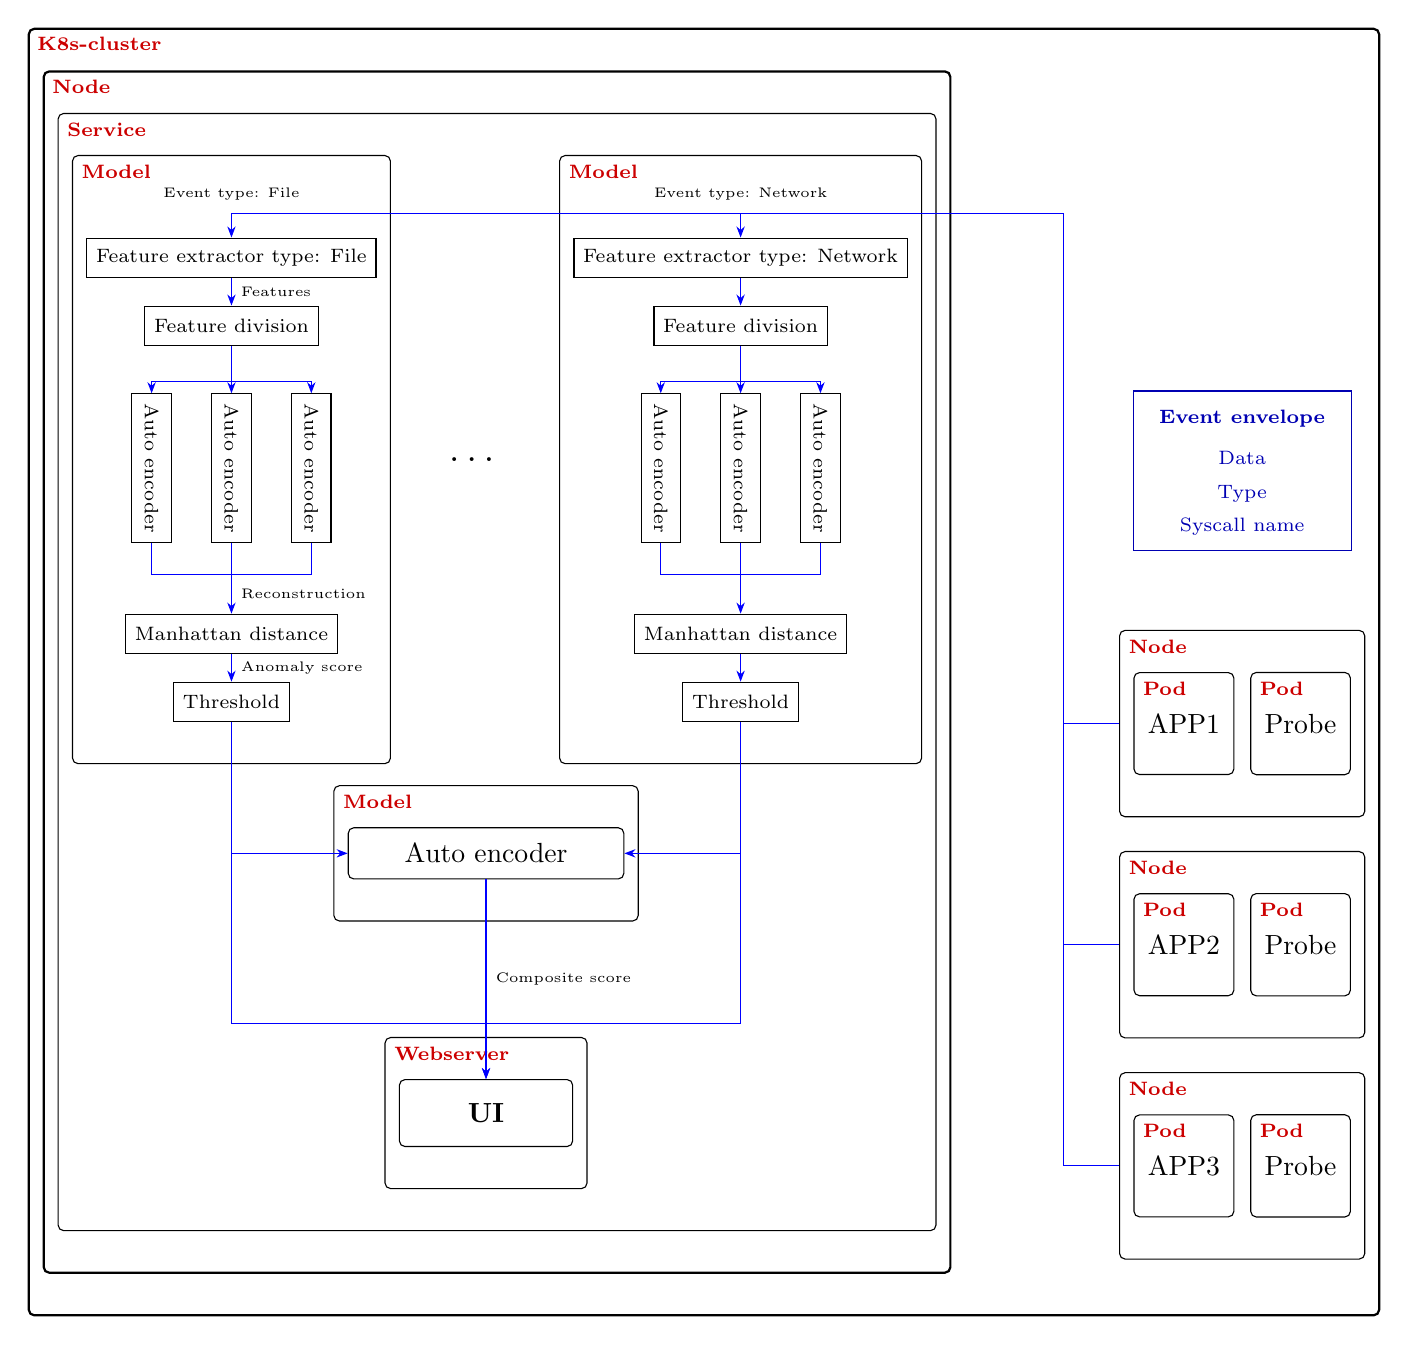
\begin{tikzpicture}[
  node distance=0.35cm and 0.5cm,
  box/.style={draw, rectangle, minimum height=0.5cm, minimum width=1cm, align=center, font=\scriptsize},
  bigbox/.style={draw, rectangle, rounded corners=2pt},
  typelabel/.style={text=red!80!black, font=\scriptsize\bfseries},
  arrow/.style={-{Stealth[length=4pt]}, draw=blue, font=\tiny},
  line/.style={draw=blue, font=\tiny},
]

  % === Top service content (left column - feature extraction) ===
  \node[box] (fe1) {Feature extractor type: File};
  % Invisible box above file feature extractor (included in model fit)
  \node[inner sep=0pt, minimum size=0pt, draw=none, above=0.5cm of fe1] (fe1top) {};
  \node[box, below=of fe1] (fdiv) {Feature division};
  % Three auto encoder boxes next to each other with vertical text,
  % AE2 centered under the feature division.
  \node[box, minimum width=0.5cm, minimum height=0.9cm,
        below=0.6cm of fdiv] (ae2) {\rotatebox{-90}{\scriptsize Auto encoder}};
  \node[box, minimum width=0.5cm, minimum height=0.9cm,
        left=0.5cm of ae2] (ae1) {\rotatebox{-90}{\scriptsize Auto encoder}};
  \node[box, minimum width=0.5cm, minimum height=0.9cm,
        right=0.5cm of ae2] (ae3) {\rotatebox{-90}{\scriptsize Auto encoder}};
  \node[box, below=0.9cm of ae2] (md) {Manhattan distance};
  \node[box, below=of md] (thresh) {Threshold};

  % Model box around feature extractor, division, auto encoders, managed distance and threshold
  \typeboxnode[fit=(fe1top)(fe1)(fdiv)(ae1)(ae2)(ae3)(md)(thresh)]{modelbox}{Model}{}

  % Second model (copy of the first) to the right, replacing FE2
  \node[box, right=2.5cm of fe1] (fe2) {Feature extractor type: Network};
  % Invisible box above network feature extractor (included in second model fit)
  \node[inner sep=0pt, minimum size=0pt, draw=none, above=0.5cm of fe2] (fe2top) {};
  \node[box, below=of fe2] (fdivb) {Feature division};
  \node[box, minimum width=0.5cm, minimum height=0.9cm,
        below=0.6cm of fdivb] (ae2b) {\rotatebox{-90}{\scriptsize Auto encoder}};
  \node[box, minimum width=0.5cm, minimum height=0.9cm,
        left=0.5cm of ae2b] (ae1b) {\rotatebox{-90}{\scriptsize Auto encoder}};
  \node[box, minimum width=0.5cm, minimum height=0.9cm,
        right=0.5cm of ae2b] (ae3b) {\rotatebox{-90}{\scriptsize Auto encoder}};
  \node[box, below=0.9cm of ae2b] (md2) {Manhattan distance};
  \node[box, below=of md2] (thresh2) {Threshold};
  \typeboxnode[fit=(fe2top)(fe2)(fdivb)(ae1b)(ae2b)(ae3b)(md2)(thresh2)]{modelbox2}{Model}{}

  % Ellipsis between the two models
  \path (modelbox.east) -- (modelbox2.west) node[midway, font=\Large] {\ldots};

  % Auto-encoder inside service, centered under the two models
  \path (modelbox.south) -- (modelbox2.south) coordinate[midway] (modelsMid);
  \node[bigbox, below=0.8cm of modelsMid, minimum width=3.5cm, minimum height=0.65cm] (autenc) {Auto encoder};
  \typeboxnode[fit=(autenc)]{autencbox}{Model}{}

  % === UI ===
  \node[bigbox, minimum width=2.2cm, minimum height=0.85cm,
        below=2cm of autencbox.south] (ui) {\textbf{UI}};
  \typeboxnode[fit=(ui)]{webserverbox}{Webserver}{}

  % Top service container (now also includes auto-encoder)
  \typeboxnode[fit=(modelbox)(modelbox2)(autencbox)(webserverbox)]{topservice}{Service}{}

  % Model types label
  \node[font=\tiny, above=0.35cm of fe1] {Event type: File};

  \node[font=\tiny, above=0.35cm of fe2] {Event type: Network};

  % === Application nodes (right of service) ===

  \typeboxnode[right=2.5cm of topservice.east, anchor=north west]{app1}{Pod}{APP1}%
  \typeboxnode[right=0.2cm of app1]{pb1}{Pod}{Probe}
  \typeboxnode[fit=(app1)(pb1)]{node1}{Node}{}

  \typeboxnode[below=1.5cm of app1]{app2}{Pod}{APP2}%
  \typeboxnode[right=0.2cm of app2]{pb2}{Pod}{Probe}
  \typeboxnode[fit=(app2)(pb2)]{node2}{Node}{}

  \typeboxnode[below=1.5cm of app2]{app3}{Pod}{APP3}%
  \typeboxnode[right=0.2cm of app3]{pb3}{Pod}{Probe}
  \typeboxnode[fit=(app3)(pb3)]{node3}{Node}{}



  % === Event envelope (blue, above the nodes) ===
  \node[draw=blue!70!black, text=blue!70!black, rectangle,
        minimum width=1.9cm, minimum height=1.1cm,
        above=1.0cm of node1] (envelope) {
    \begin{tabular}{c}
      \textbf{\scriptsize Event envelope} \\[3pt]
      \scriptsize Data \\ \scriptsize Type \\ \scriptsize Syscall name
    \end{tabular}
  };

  \typeboxnode[draw=black, thick,
  fit=(topservice)]{MainNode}{Node}{}


  % === K8s-cluster container (around everything) ===
  \typeboxnode[draw=black, thick,
               fit=(MainNode)(node1)(node2)(node3)(envelope)]{k8s}{K8s-cluster}{}

  % --- Arrows within top service (left model) ---
  \draw[arrow] (fe1) -- node[right] {Features} (fdiv);
  
  % Split 0.2cm above middle AE, directly below fdiv.south
  \coordinate (meetFdivAEy) at ($(ae2.north)+(0,0.2cm)$);
  \coordinate (meetFdivAE) at (fdiv.south |- meetFdivAEy);
  \draw[arrow] (fdiv.south) -- (meetFdivAE)  |- ($(ae1.north)+(0,0.15cm)$) -- (ae1.north);
  \draw[arrow] (meetFdivAE) |- ($(ae2.north)+(0,0.15cm)$) -- (ae2.north);
  \draw[arrow] (meetFdivAE) |- ($(ae3.north)+(0,0.15cm)$) -- (ae3.north);
  % Auto encoder outputs -> managed distance (meet 0.5cm above md)
  \coordinate (meetAEMd) at ($(md.north)+(0,0.5cm)$);
  \draw[line] (ae1.south) -- (ae1.south |- meetAEMd) |- (meetAEMd);
  \draw[line] (ae2.south) -- (ae2.south |- meetAEMd) |- (meetAEMd);
  \draw[line] (ae3.south) -- (ae3.south |- meetAEMd) |- (meetAEMd);
  \draw[arrow] (meetAEMd) -- node[right] {Reconstruction} (md.north);
  \draw[arrow] (md) -- node[right] {Anomaly score} (thresh);

  % --- Arrows within right model (from nodes) ---
  \draw[arrow] (fe2) -- (fdivb);
  \coordinate (bus3) at ($(node3.west)+(-0.7cm,0)$);
  \coordinate (bus2) at ($(node2.west)+(-0.7cm,0)$);
  \coordinate (bus1) at ($(node1.west)+(-0.7cm,0)$);
  \coordinate (busTopfe2) at ($(fe2.north)+(0,0.3cm)$);
  \coordinate (busTopFe1) at ($(fe1.north)+(0,0.3cm)$);

  \draw[line] (node3.west) -- (bus3) -- (bus2);
  \draw[line] (node2.west) -- (bus2) -- (bus1);
  \draw[line] (node1.west) -- (bus1) |- (busTopfe2);
  \draw[arrow] (busTopfe2) -- (fe2.north);
  \draw[arrow] (busTopfe2) |- (busTopFe1) -- (fe1.north);
  % Split 0.2cm above middle AE, directly below fdivb.south
  \coordinate (meetFdivbAEby) at ($(ae2b.north)+(0,0.2cm)$);
  \coordinate (meetFdivbAEb) at (fdivb.south |- meetFdivbAEby);
  \draw[arrow] (fdivb.south) |- (meetFdivbAEb) |- ($(ae1b.north)+(0,0.15cm)$) -- (ae1b.north);
  \draw[arrow] (meetFdivbAEb) |- ($(ae2b.north)+(0,0.15cm)$) -- (ae2b.north);
  \draw[arrow] (meetFdivbAEb) |- ($(ae3b.north)+(0,0.15cm)$) -- (ae3b.north);
  % Auto encoder outputs -> managed distance (meet 0.5cm above md2)
  \coordinate (meetAEbMd2) at ($(md2.north)+(0,0.5cm)$);
  \draw[line] (ae1b.south) |- (meetAEbMd2);
  \draw[line] (ae2b.south) |- (meetAEbMd2);
  \draw[line] (ae3b.south) |- (meetAEbMd2);
  \draw[arrow] (meetAEbMd2) -- (md2.north);
  \draw[arrow] (md2) -- (thresh2);

  % Thresholds -> auto-encoder (only 90° angles: vertical then horizontal)
  \draw[arrow] (thresh.south) -- (thresh.south |- autenc.west) -- (autenc.west);
  \draw[arrow] (thresh2.south) -- (thresh2.south |- autenc.east) -- (autenc.east);

  % Thresholds -> UI (meet 0.5cm above UI north, then down to UI)
  \coordinate (threshUIMeet) at ($(ui.north)+(0,0.7cm)$);
  \draw[line] (thresh.south) |- (threshUIMeet);
  \draw[line] (thresh2.south) |- (threshUIMeet);
  \draw[arrow] (threshUIMeet) -- (ui.north);

  % Auto-encoder -> UI
  \draw[arrow] (autenc.south) -- node[right] {Composite score} (ui.north);

\end{tikzpicture}
\end{document}
